\documentclass[letterpaper]{article} 
\usepackage[left = 0.5in, right = 0.5in, top = 0.9in, bottom = 0.9in]{geometry}
\usepackage{enumitem}
\usepackage{multicol}
\usepackage[spanish]{babel}
\usepackage[utf8]{inputenc}

\usepackage{amsmath,amssymb,amsthm}
\usepackage{tikz-cd}
\usepackage{mathrsfs}
\usepackage[bbgreekl]{mathbbol}
\usepackage{dsfont}
\usepackage{graphicx}
\graphicspath{{img/}}

\newcommand{\op}{\operatorname}
\newcommand{\Op}{^{\op{op}}}
\newcommand{\scc}{\mathscr C}
\newcommand{\scd}{\mathscr D}
\newcommand{\sce}{\mathscr E}
\newcommand{\sci}{\mathscr I}
\newcommand{\scj}{\mathscr J}
\newcommand{\scx}{\mathscr X}
\newcommand{\var}{\mathrm{Var}}
\newcommand{\Id}{\operatorname{Id}}
\newcommand{\N}{\mathbb N}
\newcommand{\Z}{\mathbb Z}
\newcommand{\Q}{\mathbb{Q}}
\newcommand{\I}{\mathbb{I}}
\newcommand{\R}{\mathbb{R}}
\newcommand{\C}{\mathbb{C}}
\newcommand{\F}{\mathcal{F}}
\newcommand{\G}{\mathcal{G}}
\newcommand{\B}{\mathcal{B}}
\newcommand{\abs}[1]{\left\lvert #1 \right\rvert}
\newcommand{\inv}{^{-1}}
\renewcommand{\to}{\rightarrow}
\newcommand{\ent}{\Longrightarrow}
\newcommand{\E}{\mathbb{E}}
\renewcommand{\P}{\mathbb{P}}
\newcommand{\1}{\mathds{1}}
\renewcommand{\qedsymbol}{$\blacksquare$}

\theoremstyle{definition}
\newtheorem{dfn}{Definición}
\theoremstyle{definition}
\newtheorem{teo}{Teorema}
\theoremstyle{definition}
\newtheorem{cor}{Corolario}
\theoremstyle{definition}
\newtheorem{prop}{Proposición}
\theoremstyle{definition}
\newtheorem{obs}{Observación}


\title{\textbf{Cómputo Científico\\
Tarea 3\\   
Estabilidad}}
\author{Iván Irving Rosas Domínguez}
\date{\today}

\DeclareSymbolFontAlphabet{\mathbbm}{bbold}
\DeclareSymbolFontAlphabet{\mathbb}{AMSb}
\DeclareMathSymbol\bbDelta  \mathord{bbold}{"01}

\begin{document}
\maketitle

%\begin{abstract}
%\end{abstract}

\begin{enumerate}
    \item [\textbf{1.}] Sea $Q$ una matriz unitaria aleatoria de $20\times20$ (eg. con $A$ una matriz
    de tamaño $20\times 20$ aleatoria calculen su descomposición $QR$). Sean $\lambda_1>\lambda_2>...>\lambda_{20}=1>0$
    y 
    \[
    B=Q^*diag(\lambda_1,\lambda_2,...,\lambda_{20})Q \text{ y } B_\varepsilon=Q^*diag(\lambda_1+\varepsilon_1,\lambda_2+\varepsilon_2,...,\lambda_{20}+\varepsilon_{20})Q,
    \]
    con $\varepsilon_i\sim N(0,\sigma)$, con  $\sigma=0.02$ y $\lambda_{20}=1$.
    \begin{enumerate}
        \item Comparar la descomposición de Cholesky de $B$ y de $B_\varepsilon$ usando 
        el algoritmo de la tarea 1. Considerar los casos cuando $B$ tiene un 
        $buen$ número de condición y un $mal$ número de condición.\\

        \textbf{Solución:} este ejercicio está resuelto computacionalmente en el script 'Ejercicio 1'. Para la solución de este ejercicio, simulamos una matriz aleatoria $U$ cuyas entradas sean uniformes
        en el intervalo $(-5,5)$. Le realizamos la descomposición $QR$, y seleccionamos la matriz $Q$ que por construcción es unitaria.
        Después de ello, construimos de manera adecuada la matriz de eigenvalores, para el caso bien condicionado y para el caso mal condicionado
        Para ello, definimos:
        \[
          \lambda_i:=\frac{a^{20}}{a^{i}}, \quad i\in \{1,...,20\},  
        \]
        donde $a$ es una constante que se define más adelante. De esta manera, nuestros eigenvalores forman una sucesión geométrica, y
        por construcción, $\lambda_20=1$, así como $\lambda_1=a^{20}$. Luego, el número de condición de la matriz $B$ que se forme con 
        estos valores como eigenvalores al hacer el producto $Q^t\dot diag\cdot Q$, tendrá número de condición $K(B)=\lambda^{20}=a^{20}$.\\

        Con lo anterior en mente, construimos una matriz $B1$ bien condicionada seleccionando $a=1.1$. Entonces la matriz $B1$ resultante tiene
        como número de condición $K(B1)\approx6.1159$. Asimismo, construimos una matriz $B2$ mal condicionada seleccionando $a=7$, resultando
        en que el número de condición de esta matriz es $K(B2)=\approx1.13988x10^{16}$, el cual es enorme.\\

        Creamos finalmente una matriz diagonal tal que los elementos de la diagonal sean aleatorias con media cero y desviación $\sigma=0.02$ como
        se especifica. Creamos posteriormente las matrices $B1_{}err$ y $B2_{}err$ con los errores añadidos a la matriz diagonal que posee los
        eigenvalores construidos.\\

        Con las matrices $B1,B1_{}err,B2$ y $B2_{}err$, realizamos las descomposiciones de Cholesky para realizar comparaciones. En nuestro análisis
        hacemos un paso intermedio antes de comparar: el algoritmo implementado de Cholesky no retorna una matriz triangular superior, sino que
        incluye dentro de sí restos de cálculos en la parte inferior. Dado que lo que nos importa es la precisión de la parte útil, procedemos
        a crear una función $ReChol$, la cual está cargada al inicio del script y que elimina la 'basura' de la descomposición de Cholesky que
        se implementó.\\

        Ya con las matrices limpias, realizamos 4 pruebas de comparación:
        \begin{enumerate}
            \item La prueba 1 consiste en extraer la norma $\infty$ inducida de la diferencia entre la descomposición de Cholesky de la matriz $B1$ y la de $B1_{}err$.
            Estas matrices tienen por nombre $Zc$ y $Wc$ respectivamente en los scripts, es decir encontramos $\|Zc-Wc\|_{\infty}$. hacemos
            lo análogo para las matrices $B2$ y $B2_{}err$, cuyos nombres son $Xc$ y $Yc$ en el script, respectivamente. Para ello se utiliza la función $np.max(abs(Zc-Wc))$.
            \item La prueba 2 consiste en extraer la norma $2$ inducida de la misma diferencia anterior, es decir, $\|Zc-Wc\|_{2}$ para el
            caso bien condicionado, y lo análogo para el mal condicionado. Para ello se utiliza la función $np.linalg.norm(-,ord=2)$.
            \item La prueba 3 consiste en extraer la norma $\infty$ pero ahora de la diferencia entre la matriz $B1$ o $B2$ que se recuperan al multiplicar las descomposiciones
            Cholesky apropiadamente, con las matrices $B1$ o $B2$ originales respectivamente. La idea de esta prueba es que, después de todo,
            la descomposición de Cholesky debe darnos la posibilidad de poder recuperar la matriz original correctamente.
            \item La prueba 4 consiste en extraer la norma 2 inducida de la diferencia anterior.
        \end{enumerate}
        Con lo anterior dicho, procedemos a realizar las pruebas. Los resultados son los obtenidos en la siguiente figura.
        \begin{figure}[h]
            \centering
            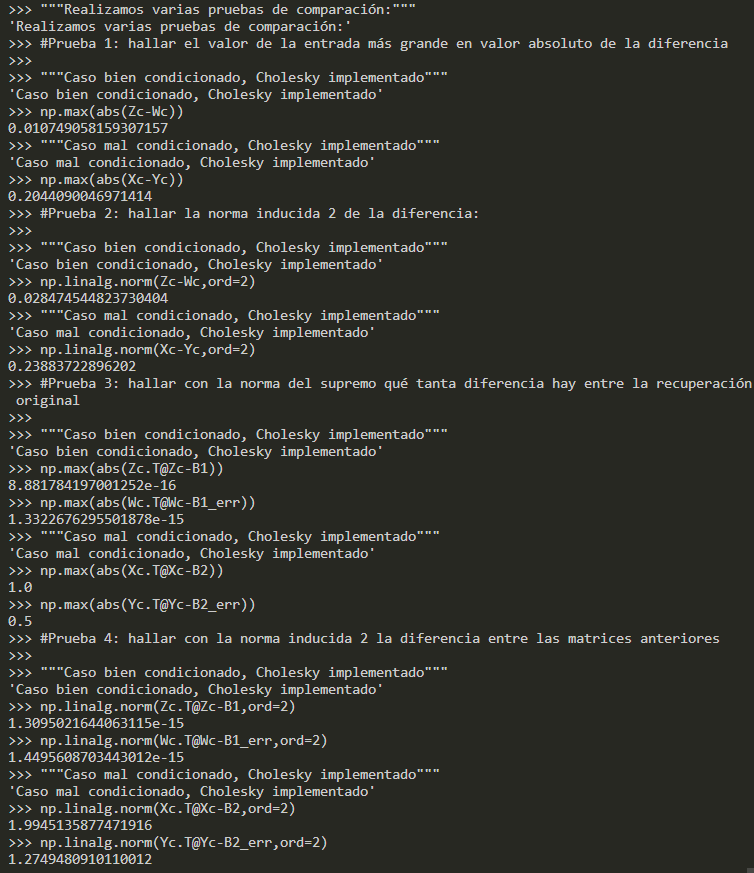
\includegraphics[width=0.7\linewidth]{3.png}
            \caption{Comparación de las 4 pruebas realizadas, cholesky implementado, caso bien condicionado vs caso mal condicionado.}
        \end{figure}
        Como se puede observar, en la prueba 1, el tamaño más grande de la matriz diferencia $B1-B1_{}err$ es de aproximadamente $0.0107$ para
        el caso bien condicionado, mientras que en el mal condicionado, el tamaño de $B2-B2_{}err$ es de aproximadamente $0.2044$, lo cual procedemos
        decir que es 20 veces más que el error de la bien condicionada.\\

        En la prueba 2, la norma 2 inducida de la diferencia en el caso bien condicionado es de $0.02847$, mientras que 
        en el caso mal condicionado es de $0.2388$ aproximaddamente, lo cual nos dice que la norma de la diferencia es 10 veces
        más grande en el caso mal condicionado que en el bien condicionado.\\

        Realizamos la tercera prueba, para el caso bien condicionado, en norma $\infty$, 
        tanto la matriz $B1$ como $B1_{}err$ recuperadas difieren de la original $B1$ en $8.8817\times 10^{-16}$ y $0.01845$ aproximadamente,
        es decir, se recupera muy bien la matriz $B1$ cuando no hay error, y cuando se le sumó el error $Delta$, ciertamente la diferencia es
        del orden de 0.01845, pero sigue siendo pequeño.
        \newline

        Para el caso mal condicionado, esta prueba arroja $1$ para la distancia con norma $\infty$ entre $B2$ y la recuperación,
        contrastando con el $0.5$ que arroja la distancia con norma $\infty$ entre $B2$ y la recuperación usando $B2_{}err$.
        \newline

        Finalmente, para la prueba 4 en el caso bien condicionado, la distancia con norma 2 entre $B1$ y la recuperación usando $B1$ es
        de $1.3095\times10^{-15}$, lo cual es bastante pequeño, mientras que la distancia entre $B1$ y la recuperación usando $B1_{}err$
        es de $0.03967$, que ciertamente es mayor que la anterior pero no demasiado.\\

        Sin embargo, para el caso mal condicionado, la prueba 4 arroja una distancia con normal 2 entre $B2$ y su recuperación con $B2$ mismo
        de aproximadamente 1.9945, mientras que para la recuperación utilizando $B2_{}err$, obtenemos una distancia de 
        aproximadamente 1.2849.
        \newline

        De estas pruebas podemos observar que una matriz mal condicionada, cuando se perturba un poco, en efecto termina difiriendo
        en una medida notoria de las originales.


        \item Con el caso mal condicionado, comparar el resultado de su algoritmo con el del algoritmo
        de Cholesky de scipy.\\

        \textbf{Solución:} para este ejercicio, ya tenemos las pruebas realizadas anteriormente, por lo que ahora comparamos con 
        las que cholesky de scipy nos arroja. Esto se puede ver en la figura.

        \begin{figure}[h]
            \centering
            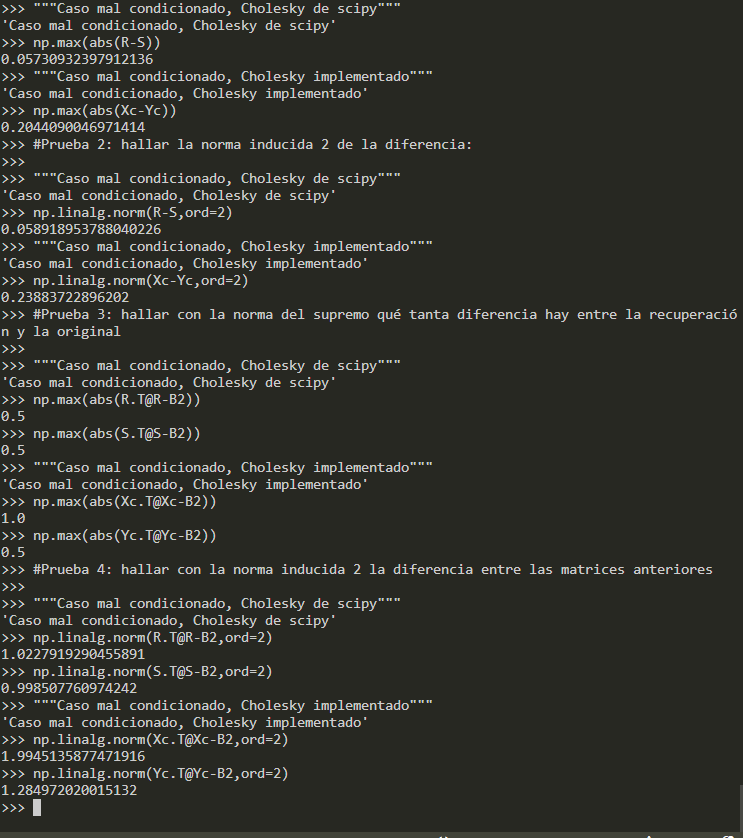
\includegraphics[width=0.7\linewidth]{4.png}
            \caption{Comparación de las 4 pruebas realizadas, cholesky implementado vs scipy en el caso mal condicionado.}
        \end{figure}

        De manera similar al análisis hecho antes, notemos que para la prueba 1, la norma infinito de la diferencia entre la descomposición de 
        la matriz $B2$ y $B2_{}err$, utilizando cholesky de scipy y el cholesky implementado nos otorga un valor de $0.0573$ y $0.204409$ aproximadamente
        y respectivamente. De aquí se infiere que es mejor, con esta métrica, el algoritmo de cholesky de scipy.
        \newline

        Para la prueba 2, utilizando la norma 2, cholesky de scipy nos otorga una norma de $0.05891$ aproximadamente, en contraste con 
        el valor de la norma 2 utilizando cholesky implementado, el cual es de $0.23883$ aproximadamente. Nuevamente concluimos que es mejor
        en este sentido el algoritmo de scipy.
        \newline

        Para la prueba 3, en el caso de scipy obtenemos que la norma infinito de la diferencia entre $B2$ y $B2$ recuperada, para
        cuando añadimos error y cuando no añadimos error en la diagonal, usando scipy, es de $0.5$ en ambos casos. Mientras que
        la norma infinito para la misma diferencia usando cholesky implementado es de $1$ y $0.5$ respectivamente. Los resultados
        son similares, pero también en el caso de scipy, se obtiene un mejor resultado.\\

        Finalmente en la prueba 4, se tiene que la norma 2 inducida de la diferencia entre $B2$ y su recuperación usando scipy es
        de $1.0227$ y $0.9985$ aproximadamente, en los casos donde no se agrega error y sí se agrega error en las diagonales, 
        respectivamente. Esto contrasta con los valores $1.99451$ y $1.2849$ obtenidos antes para el algoritmo de Cholesky implementado.
        Concluimos de estas cuatro pruebas que en el caso mal condicionado, Cholesky de scipy tiene un mejor desempeño en la minimización
        de las diferencias entre las normas de las matrices.

        \item Medir el tiempo de ejecución de su algoritmo de Cholesky con el de scipy.
        \item \textbf{Solución:} Dado que si solamente descomponemos una vez la matriz, los tiempos 
        son demasiado pequeños para ser de interés, realizamos 500 veces la descomposición de la matriz
        $B2$ y comparamos los tiempos de ejecución de esas 500 operaciones. Los resultados se pueden ver
        en la siguiente figura:

        \begin{figure}[h]
            \centering
            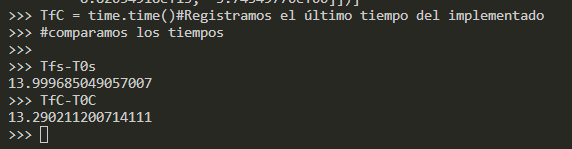
\includegraphics[width=0.7\linewidth]{5.png}
            \caption{Comparación de los tiempos de ejecución de scipy vs la implementación.}
        \end{figure}
        Nuevamente volvemos a comprobar que el algoritmo de scipy es mejor, esta vez en el rubro de los tiempos, ya que
        aunque la diferencia es ligera, es más rápida la descomposición de scipy que la implementada por 70 ms aproximadamente.
        \end{enumerate}

    \item [\textbf{2.}] Resolver el problema de mínimos cuadrados,
        \[
        y=X\beta+\varepsilon, \quad \varepsilon_i\sim N(0,\sigma),
        \]
        usando su implementación de la descomposición $QR$; $\beta$ es de tamaño $d\times 1$ y $X$ de tamaño
        $n\times d$. \\
        Sean $d=5$, $n=20$, $\beta=(5,4,3,2,1)^t$ y $\sigma=0.13$.
        \begin{enumerate}
            \item Hacer $X$ con entradas aleatorias $U(0,1)$ y simular $y$. Encontrar $\hat{\beta}$ y 
            compararlo con el obtenido $\hat{\beta}_p$ haciendo $X+\Delta X$, donde las entradas de
            $\Delta X$ son $N(0,\sigma)$,  $\sigma=0.01$. Comparar a su vez con $\hat{\beta}_c=\left(\left(X+\Delta X\right)^t\left(X+\Delta X\right)\right)^{-1}(X+\Delta X)^ty$,
            usando el algoritmo genérico para invertir matrices scipy.linalg.inv.
            \newline

            \textbf{Solución:} este ejercicio se encuentra resuelto computacionalmente en el script titulado 'Ejercicio 2'. Para resolverlo,
            tal y como se muestra en el código, se importan primero las paqueterías a usar, las cuales
            son numpy, y scipy.stats.norm, uniform, así como scipy.linalg.inv, para calcular la inversa
            de las matrices. Se importan asimismo los algoritmos necesarios para hallar el estimador
            de mínimos cuadrados de la tarae pasada.\\

            Ahora bien, procedemos colocando una semilla $n=15$ para poder replicar resultados. Procedemos a crear la aleatoria $X$ de tamaño $20\times5$ 
            con entradas uniformes en (0,1). También creamos una matriz de error, $Delta$, guardamos la matriz $X+\Delta X$ como $Xerr$ y finalmente
            creamos un vector $e$ de errores normales como se indica. 
            \newline

            Para revisar el estado de las matrices, hallamos su número de condición utilizando
            la función $np.linalg.cond()$. El resultado es el siguiente:
            \begin{verbatim*}
                >>> np.linalg.cond(X)
7.44759999264605
>>> np.linalg.cond(Xerr)
7.511998266815689
            \end{verbatim*}
            de tal forma que la matriz $X$ y $Xerr$ son ambas matrices bien condicionadas, ya que
            sú número de condición es relativamente pequeño.\\

            Se simula el vector de observaciones $y$ con $20$ elementos, y se halla el estimador de 
            mínimos cuadrados denotado por $bhat$, utilizando las funciones anteriormente hechas. Se
            encuentra así mismo el estimador de mínimos cuadrados, denominado $bhat_p$ para la matriz $Xerr$ con las observaciones
            $y$ y también se encuentra el estimador de mínimos cuadrados teórico utilizando la matriz $Xerr$,
            denotado por $bhat_c$. Los resultados se encuentran a continuación:

    \begin{figure}[h]
        \centering
        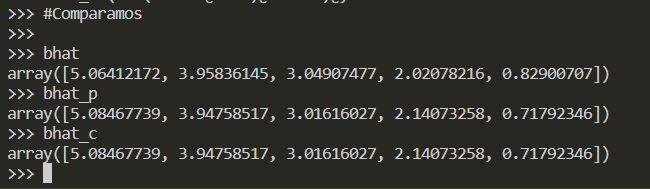
\includegraphics[width=0.7\linewidth]{0.png}
        \caption{Comparación de los tres estimadores utilizando una matriz $X$ 'bien condicionada'.}
    \end{figure}
Como se puede observar en la imagen, los resultados no son los mejores, sin embargo la estimación se
acerca bastante al vector $\beta=(5,4,3,2,1)$ de los verdaderos valores.\\

Cabe destacar que el estimador $bhat_p$ y $bhag_c$ tienen los mismos valores, esto es, 
el estimador teórico coincide con aquél hallado con la implementación para el caso de la matriz
$X+\Delta X$.
            \item Lo mismo que el anterior pero con $X$ mal condicionada (i.e. con casi colinealidad).\\
            

            \textbf{Solución:} para este caso, lo que hacemos es tomar la matriz $X$, tomar la primera
            columna, e insertarla en la columna 2, 3, 4 y 5 de una nueva matriz que llamaremos $Y$,
            multiplicadas cada una por un factor de 
            $k/3$, donde $k$ es el valor de la columna a ser rellenada. De esta manera tenemos una matriz con 
            colinealidad total. Luego, para evitar la colinealidad total, creamos una matriz que genere
            ruido y la sumamos a la matriz $Y$. La matriz de ruido tiene entradas uniformes en (0,0001), de tal
            forma que ciertamente no hay colinealidad, pero se tiene algo muy cercano.
            La matriz $Y$ con el ruido sumado se renombra como $Y$ misma.
            \newline

            Se construye la matriz $Y+Delta=Yerr$ tal y como se hizo antes, donde recordemos que las entradas
            de $\Delta$ son normales. Para comprobar que estas nuevas matrices $Y$ y $Yerr$ tienen bastante colinealidad, se calcula el número
            de condición como se hizo antes, y se obtiene que
            \begin{verbatim*}
                >>> np.linalg.cond(Y)
74804.68813239328
>>> np.linalg.cond(Yerr)
276.91509065873987
>>>.
            \end{verbatim*}
            Estos valores ya nos dicen algo interesante: la matriz a la que no se le está
            sumando el ruido $Delta$, luego de realizar el procedimiento anterior, 
            tiene un número de condición grande, mientras que aquella que sí se le está sumando, 
            tiene uno más pequeño. Esto quiere decir que la matriz $Y$ va a alterar mucho más los valores
            de salida al realizar opearciones con ella, mientras que la matriz $Yerr$ no tanto, a pesar
            de que está formada con un error.
            \newline

            Pero lo anterior es explicable gracias a que, justamente al añadir el término $Delta$ a 
            la matriz $Y$, esta pierde más aún la colinealidad, de tal forma que su número de condición 
            mejora.
            \newline

            Procedemos a simular el vector de valores observados que ahora denotamos por $z$ (este vector
            tiene como matriz de diseño a la matriz $Y$, y no a $X$), y con ello, se encuentran los tres
            estimadores. Los resultados se muestran en la figura 2.

            \begin{figure}[h]
                \centering
                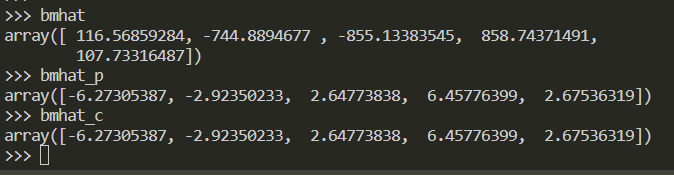
\includegraphics[width=0.7\linewidth]{1.png}
                \caption{Comparación de los tres estimadores utilizando una matriz $Y$ 'con casi colinealidad'.}
            \end{figure}
            Nótese que los estimadores de mínimos cuadrados se vuelven absurdos en el caso de la matriz $Y$, mientras
            que en el caso de la matriz $Yerr$, los estimadores también son malos, pero presentan un comportamiento
            menos caótico y ciertamente sus valores son  más cercanos a los valores de los estimadores reales
            que aquellos de los estimadores creados ocn la matriz $Y$.\\

            Esto concuerda totalmente con lo observado en el número de condición de la matriz $Y$ y $Yerr$: el 
            error que es añadido por la matriz $Delta$ distorsiona adecuadamente a $Y$ de tal forma que $Yerr$
            resulta arrojar mejores resultados computacionales que $Y$ misma.\\

            Finalmente, los estimadores $bmhat_p$ y $bmhat_c$ coinciden nuevamente, así como 
            lo hicieron en el caso de la matriz $X$ bien condicionada.
\end{enumerate}
\end{enumerate}
\end{document}